\begin{document}
%=================================================================
%                           Start Document
%=================================================================
\section{System Design}
\lhead{System Design} % section header

\setstretch{1.6}


\subsection{Functional Electrical Stimulation}

\subsubsection{Electrode configuration}
There are two main configuration for electrical activation of neuromuscular tissue. There is bipolar stimulation in which each stimulation cite has an active electrode placed near the peripheral nerve and a reference electrode close by. The other configuration is monopolar where the return electrode is placed in a remote area near less excitable tissue \cite{peckham_functional_2005}. 
This approach reduces the number of leads and electrodes required, however for multichannel systems bipolar stimulation may allow greater selectivity of activation because each electrode par creates a more localized electric field \cite{grandjean_recruitment_1986}. 

\subsubsection{Stimulation waveform}
Stimulus waveforms are generally monophasic or biphasic. Monophasic waveforms consist of a single phase of electrical current delivered in one polarity, while Biphasic waveforms consist of a cathodic phase followed by an anodic phase. This mitigates the buildup of charge at the electrode-tissue interface by ensuring that the net charge delivered over time is zero, effectively reducing the risk of tissue damage as compared to monophasic waveforms \cite{peckham_functional_2005}. Additionally the biphasic rectangular stimulation is the most commonly used, as it offers the best force-amplitude ratio
\cite{lynch_functional_2008}. For these reasons the balanced biphasic rectangular waveform was chosen for the stimulation protocol.
 \begin{figure} [H]
     \centering
     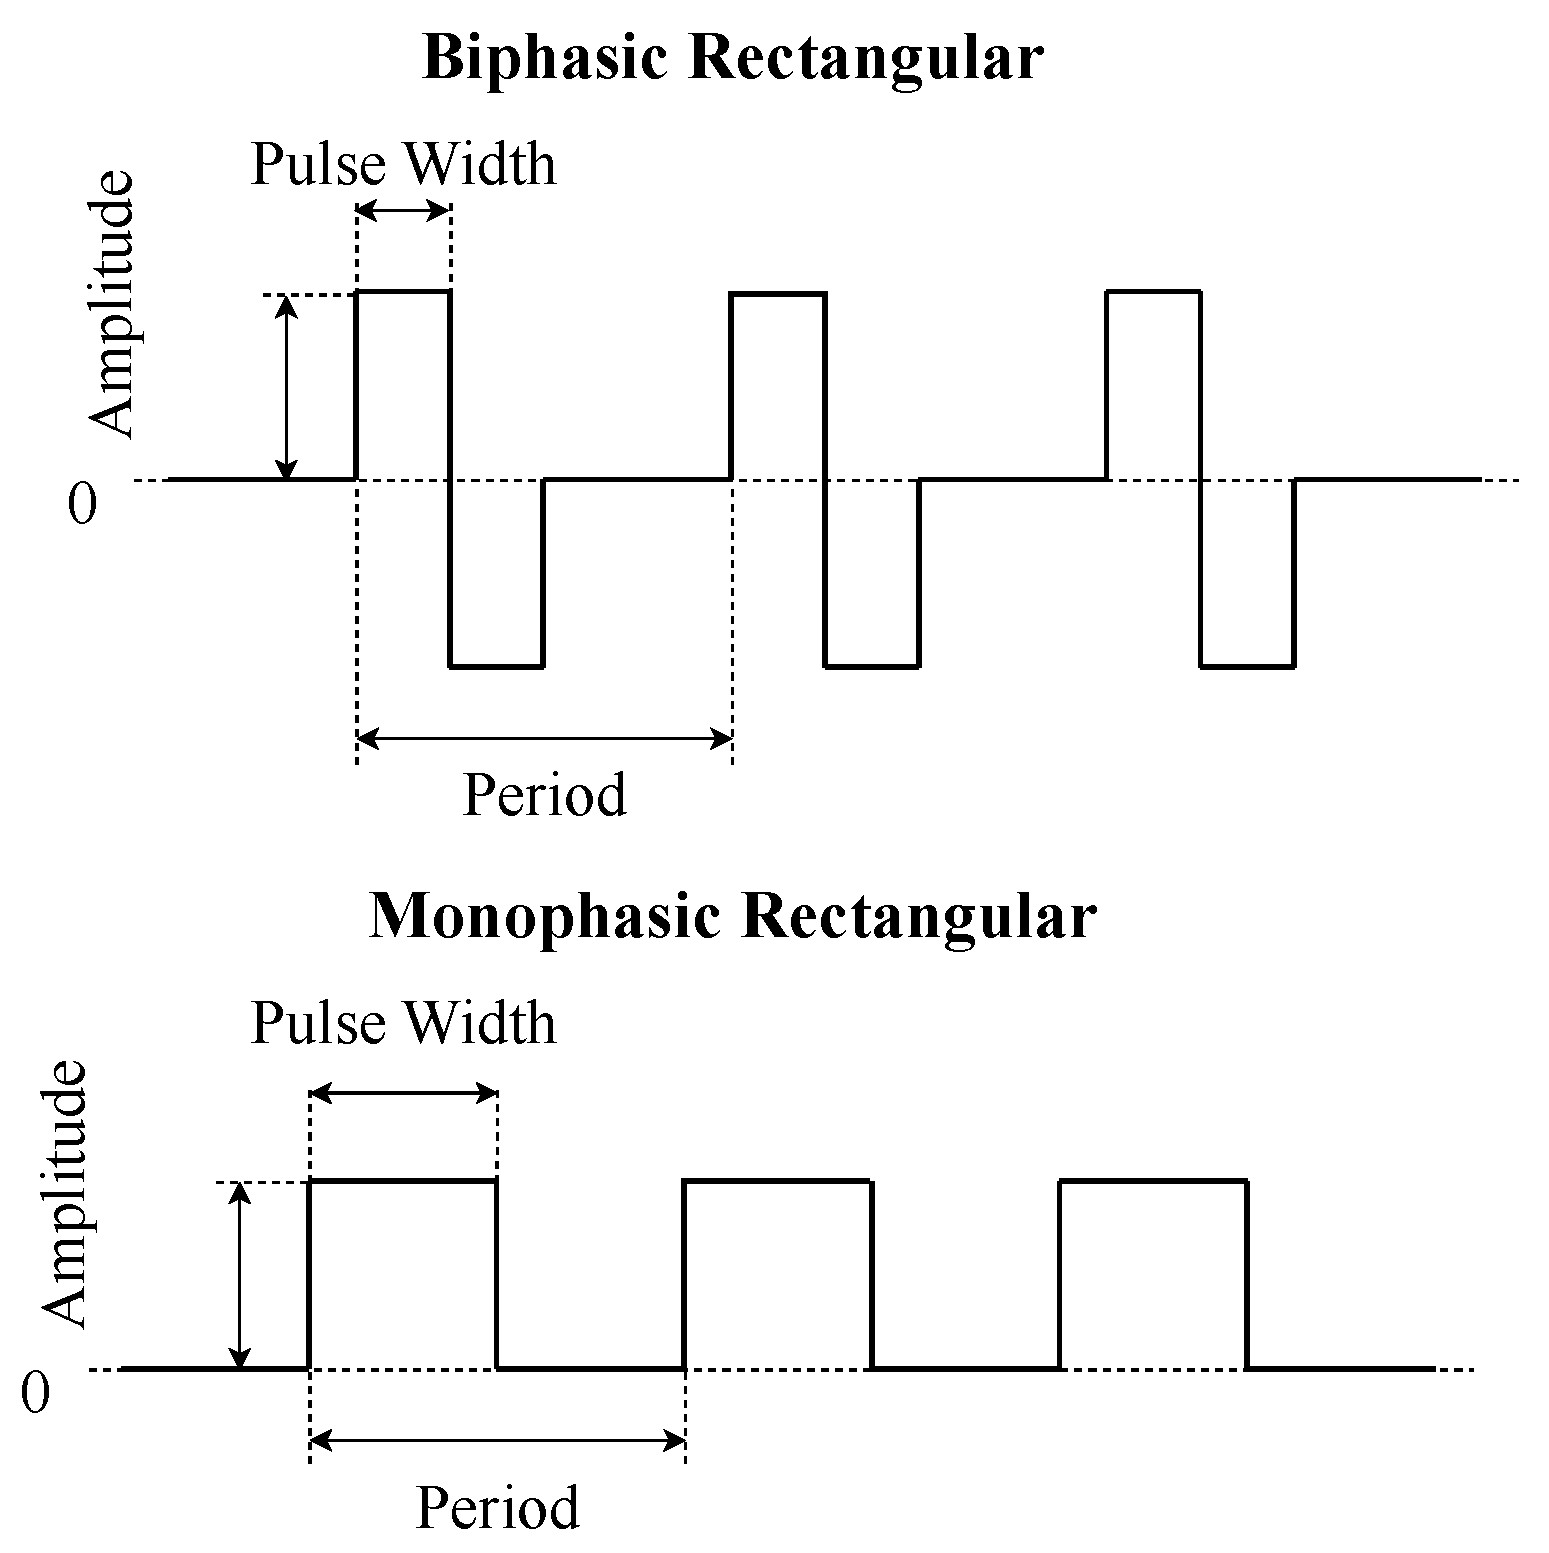
\includegraphics[width=0.6\linewidth]{images/twowaveform.jpg}
     \caption{Caption}
     \label{fig:enter-label}
 \end{figure}

\subsubsection{Stimulation frequency}
The stimulation frequency affects the strength of the contraction and its quality. A higher frequency will lead to the force produced by each subsequent pulse being added so that the mean force of the contraction is greater than that produced by a single twitch. Further increase in frequency results in sustained contraction which produces a smooth movement instead of individual twitches. The minimum frequency required to induce fairly consistent contraction is between 16 and 20 Hz \cite{marquez-chin_functional_2020}. A smoother contraction is also more comfortable for the patient. However one should not use a higher frequency than necessary since it has been observed that fatigue accumulated in a muscle is related to the number of pulses received \cite{bigland-ritchie_muscle_2000}. 

\begin{figure} [H]
    \centering
    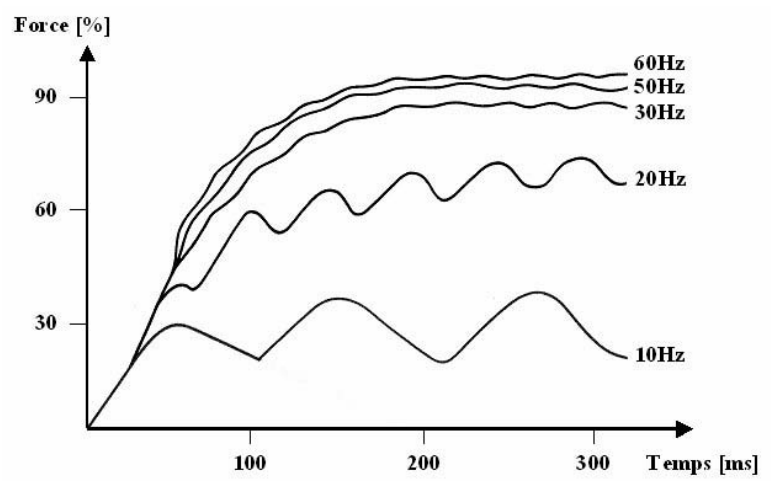
\includegraphics[width=0.7\linewidth]{images/stimfreq.png}
    \caption{Effect of stimulation frequency on force generation \cite{metrailler_systeme_2005}}
    \label{fig:enter-label}
\end{figure}

When choosing the stimulation frequency the aim was therefore to choose the lowest frequency that still produced sustained contractions. In a clinical environment, the typical range of frequencies is around 20-50Hz, and during literature review it was observed that the majority of teams using FES on gait are using a stimulation frequency around 40Hz \cite{aout_effects_2023}. Therefore the same 40Hz stimulation frequency was chosen for this project.

\subsubsection{Stimulation intensity }
The stimulation intensity is determined by the pusle duration as well as the pulse amplitude. To vary the intesity one is therefore often kept constant while the other is tuned. 

 \todo{explain better why modulating w amplitude?} 
The pulse duration (pulse width) is the timespan of the stimulation pulse. Higher pulse widths result in more pronounced contraction and enable deeper tissue penetration of the stimulation . Most sudies attempting FES for gait employ pulse widths spanning from 200 to 400 \micro s. The majority keep the pulse duration fixed at 300 \micro s and only vary the amplitude in order to set the stimulation intensity.\cite{aout_effects_2023}

The amplitude of the stimulation determines which muscles are contracted and the strength of the contraction \cite{marquez-chin_functional_2020}. Larger amplitudes a larger proportion of the muscle fibers, including those located deeper. 



There are several clinically important values for the amplitude that can be identified. The first is the motor threshold, which is the minimum intensity  that results in a visible muscle contraction, even if it does not produce a movement \cite{marquez-chin_functional_2020}. The second is the Maximum tolerable intensity, which is the maximum amplitude that the person can sustain without pain. Finally there is the operational stimulation amplitude, which is the amplitude that produces the intended functional movement needed for the gait cycle. 

These thresholds are highly variable dependent on muscle and subject, therefore they determined experimentally by slowly ramping up the amplitude. This process is expanded upon in the FES implementation chapter.






%=================================================================
%                           End Document
%=================================================================
\end{document}